%\documentclass{article}
%\usepackage{graphicx,subfigure}
%\begin{document}

\begin{figure}[h]
  \centering
  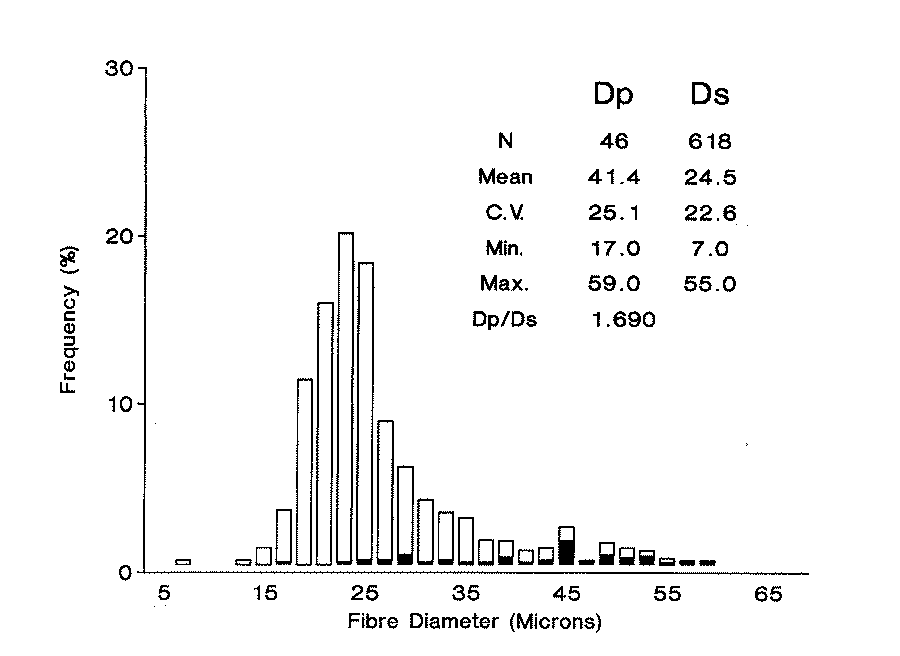
\includegraphics[width=\textwidth,trim = 0 0 0 20]{images/fig8.png}
  \caption{Fibre diameter histogram of a hogget ewe from a leading
     Australian Merino stud.  Note the high frequency of large primary
     and secondary fibres and the simultaneous presence of fine
     primary fibres.  The fine primaries are probably regrowth tips
     indicating shedding.}
  \label{fig:8}
\end{figure}

%\end{document}
